\documentclass[11pt]{article}
\usepackage[a4paper,margin=1in]{geometry}
\usepackage[T1]{fontenc}
\usepackage[utf8]{inputenc}
\usepackage{lmodern}
\usepackage{amsmath}
\usepackage{booktabs}
\usepackage{graphicx}
\usepackage{float}
\usepackage{hyperref}
\usepackage{enumitem}
\usepackage{caption}

\title{Do LLM Rankings Change if You Ask Differently?\\
\large Evaluating Ranking Reversals Under Non-semantic Prompt Perturbations and Subset Resampling}
\author{ST5230 Group 14\\
ZHANG QIANCHI \and PENG YANGYUNZHI \and JIANG YIFAN \and MENG XIANGCHEN}
\date{}

\begin{document}
\maketitle

\begin{abstract}
Static leaderboards implicitly assume that model rankings are stable under reasonable evaluation choices. We test this assumption by studying whether non-semantic prompt perturbations and evaluation-subset variation can alter model rankings on three multiple-choice benchmarks: MMLU, ARC-Challenge, and HellaSwag. We build a controlled evaluation set of 900 questions, expand it into 3,600 prompt requests using four task-preserving prompt templates, and collect 14,400 responses from GPT-4o-mini, Gemini-2.0-flash, Qwen-2.5-7B, and Llama-3.1-8B. We score all outputs automatically and use 2,000 bootstrap resamples per dataset to estimate confidence intervals, pairwise significance, and ranking reversal rate (RRR). The main finding is that ranking stability is highly benchmark-dependent. ARC-Challenge is very stable, MMLU is moderately stable with uncertainty concentrated in middle ranks, and HellaSwag is substantially less stable, with prompt-induced ranking reversals reaching 62.55\% under one prompt variant.
\end{abstract}

\section{Introduction}

Large language model evaluation is often summarized by a static leaderboard. Models are assigned benchmark scores, sorted by accuracy, and then treated as if the resulting order were a stable description of comparative ability. This is convenient, but it embeds a strong assumption: small evaluation choices should not materially change the ordering between models.

That assumption is not obviously warranted. Even when the underlying task is fixed, prompt phrasing, answer formatting, and instruction order may affect model behavior. Likewise, a reported benchmark score depends on the specific subset of items included in evaluation. If the gap between two models is small, prompt noise or sample-composition noise may be large enough to change the apparent winner.

This report studies leaderboard reliability through the lens of \textbf{ranking stability} rather than score variance alone. We ask not only whether prompt perturbations change accuracy, but whether they change the \emph{relative ordering} between models.

Our contributions are:
\begin{enumerate}[leftmargin=1.5em]
\item We evaluate ranking stability under four task-preserving prompt templates rather than a single benchmark prompt.
\item We combine prompt perturbation with bootstrap subset resampling, capturing both prompt noise and sample-composition noise.
\item We show that ranking robustness differs sharply across benchmarks: ARC-Challenge is stable, MMLU is partially stable, and HellaSwag is substantially unstable.
\end{enumerate}

\section{Related Work}

Our study is connected to three threads of prior work. First, benchmark construction papers such as MMLU, ARC, and HellaSwag established the evaluation settings used in this project and highlighted different forms of knowledge, reasoning, and commonsense difficulty. Second, prompt-robustness research has shown that large language models can be sensitive to prompt variation, even when perturbations preserve task semantics. Third, recent reliability discussions in LLM evaluation emphasize that an evaluation result is not only a property of the model, but also of the protocol used to measure it. Our project extends this perspective by focusing on whether evaluation variation is large enough to change rank order.

\section{Experimental Design}

\subsection{Benchmarks and Sampling}

We evaluate three automatically scorable multiple-choice benchmarks:
\begin{itemize}[leftmargin=1.5em]
\item \textbf{MMLU}: 300 questions, sampled as 50 questions from each of 6 subjects.
\item \textbf{ARC-Challenge}: 300 questions from the official test split.
\item \textbf{HellaSwag}: 300 questions from the validation split, because the public test split does not expose gold labels.
\end{itemize}
This yields a master sample of 900 questions.

\subsection{Prompt Templates}

Each question is transformed into four task-preserving prompt templates:
\texttt{minimal\_instruction}, \texttt{benchmark\_style}, \texttt{natural\_style}, and \texttt{order\_phrasing\_variation}. These templates preserve task semantics and answer options while varying tone, presentation, and instruction order. Expanding 900 questions by 4 templates produces 3,600 prompt requests.

\subsection{Models and Inference}

We evaluate four models:
\begin{itemize}[leftmargin=1.5em]
\item \texttt{openai/gpt-4o-mini}
\item \texttt{google/gemini-2.0-flash-001}
\item \texttt{qwen/qwen-2.5-7b-instruct}
\item \texttt{meta-llama/llama-3.1-8b-instruct}
\end{itemize}

Applying these models to 3,600 prompt requests produces 14,400 responses. All responses are generated through OpenRouter with \texttt{temperature = 0} and \texttt{max\_tokens = 150}. Outputs are parsed automatically into one of \texttt{A/B/C/D} and compared with the gold label to yield a binary score. Out of 14,400 responses, only 3 parse failures occur (0.02\%), all from Llama safety refusals.

\subsection{Bootstrap Analysis and RRR}

For each dataset, we run 2,000 bootstrap iterations. In each iteration, we sample items with replacement from the dataset and recompute prompt-specific accuracy, prompt-averaged accuracy, pairwise model differences, and rankings under each prompt template. We form 95\% confidence intervals using the 2.5th and 97.5th percentiles of the bootstrap distribution.

We take \texttt{minimal\_instruction} as the baseline prompt. In each bootstrap iteration, we compare the model ranking under each alternative prompt with the baseline ranking. If the order differs at any position, that iteration counts as a ranking reversal. The Ranking Reversal Rate (RRR) is the proportion of iterations with a changed ranking.

\section{Main Results}

\subsection{Prompt-averaged Accuracy}

Table~\ref{tab:accuracy} reports prompt-averaged accuracy and 95\% confidence intervals.

\begin{table}[H]
\centering
\caption{Prompt-averaged accuracy by dataset and model.}
\label{tab:accuracy}
\begin{tabular}{llccc}
\toprule
Dataset & Model & Accuracy & 95\% CI & Rank \\
\midrule
ARC-Challenge & Gemini-2.0-flash & 94.00\% & [91.42, 96.50] & 1 \\
ARC-Challenge & GPT-4o-mini & 90.83\% & [87.58, 93.75] & 2 \\
ARC-Challenge & Qwen-2.5-7B & 85.08\% & [81.17, 88.92] & 3 \\
ARC-Challenge & Llama-3.1-8B & 77.33\% & [73.25, 82.00] & 4 \\
HellaSwag & GPT-4o-mini & 89.17\% & [86.00, 92.09] & 1 \\
HellaSwag & Gemini-2.0-flash & 87.25\% & [84.08, 90.25] & 2 \\
HellaSwag & Qwen-2.5-7B & 84.25\% & [80.83, 87.75] & 3 \\
HellaSwag & Llama-3.1-8B & 68.33\% & [63.92, 72.75] & 4 \\
MMLU & Gemini-2.0-flash & 85.08\% & [81.17, 88.58] & 1 \\
MMLU & GPT-4o-mini & 73.42\% & [68.67, 78.17] & 2 \\
MMLU & Qwen-2.5-7B & 70.33\% & [65.58, 75.17] & 3 \\
MMLU & Llama-3.1-8B & 60.08\% & [55.08, 65.25] & 4 \\
\bottomrule
\end{tabular}
\end{table}

At the point-estimate level, Gemini leads on ARC-Challenge and MMLU, while GPT-4o-mini leads on HellaSwag. However, the stability of these rank claims differs sharply by benchmark.

\subsection{Ranking Reversal Rate}

Table~\ref{tab:rrr} reports RRR relative to the minimal prompt.

\begin{table}[H]
\centering
\caption{Ranking reversal rate relative to \texttt{minimal\_instruction}.}
\label{tab:rrr}
\begin{tabular}{lccc}
\toprule
Dataset & Benchmark & Natural & Order/Phrasing \\
\midrule
ARC-Challenge & 4.70\% & 1.65\% & 1.05\% \\
HellaSwag & 62.55\% & 41.35\% & 38.50\% \\
MMLU & 19.60\% & 8.05\% & 13.50\% \\
\bottomrule
\end{tabular}
\end{table}

The result is not a small uniform effect. ARC-Challenge is highly stable. MMLU is moderately stable. HellaSwag is markedly unstable, with reversals in more than 60\% of bootstrap iterations under the benchmark-style prompt.

\subsection{Pairwise Significance}

Pairwise bootstrap analysis shows where uncertainty is concentrated:
\begin{itemize}[leftmargin=1.5em]
\item \textbf{ARC-Challenge}: every pairwise comparison is significant at the 95\% level.
\item \textbf{HellaSwag}: GPT-4o-mini exceeds Gemini by only 1.92\%, with 95\% CI [-0.67, 4.75] and $p=0.169$.
\item \textbf{HellaSwag}: Gemini exceeds Qwen by 3.00\%, with 95\% CI [-0.58, 6.42] and $p=0.102$.
\item \textbf{MMLU}: Gemini exceeds GPT by 11.67\%, with 95\% CI [6.99, 16.08].
\item \textbf{MMLU}: GPT exceeds Qwen by 3.08\%, with 95\% CI [-1.50, 7.58] and $p=0.184$.
\end{itemize}

These results show that ranking instability is most likely when performance gaps are narrow.

\section{Benchmark-wise Analysis}

\subsection{ARC-Challenge: Stable Leaderboard}

ARC-Challenge is the most stable benchmark in the study. Gemini remains first under all prompt variants, and all pairwise gaps are significant. The low RRR values imply that prompt perturbation and subset resampling are too weak to overturn the ranking.

\subsection{HellaSwag: Fragile Top Rank}

HellaSwag is the clearest counterexample to the assumption that static leaderboards are robust. GPT-4o-mini has the highest point estimate, but its lead over Gemini is not statistically significant. At the same time, HellaSwag shows the highest RRR under every non-baseline prompt.

\subsection{MMLU: Stable Winner, Unstable Middle}

MMLU presents a mixed pattern. Gemini is clearly first and remains first across prompts. However, GPT-4o-mini and Qwen are not significantly separated, so the middle of the ranking is not fully settled.

\section{Subject-level MMLU Analysis}

We further run a subject-aware bootstrap analysis for MMLU. Pooled and stratified full-MMLU bootstrap produce the same overall order:
\[
\text{Gemini-2.0-flash} > \text{GPT-4o-mini} > \text{Qwen-2.5-7B} > \text{Llama-3.1-8B}.
\]
At the subject level, instability varies dramatically. The mean RRR across non-minimal prompts ranges from 14.50\% for high-school macroeconomics to 67.93\% for philosophy, showing that ranking robustness is not only benchmark-dependent but also subdomain-dependent.

\section{Discussion and Limitations}

Our findings support three claims. First, prompt sensitivity should not be reduced to score fluctuation alone. On some tasks, the fluctuation is large enough to alter relative ranking. Second, single-prompt evaluation can be misleading. On HellaSwag in particular, the apparent top model changes from ``plausibly best'' to ``statistically unresolved'' once prompt and subset variation are taken seriously. Third, confidence intervals on accuracy are necessary but insufficient: what often matters is whether order is robust.

This study also has clear limitations. We evaluate only three multiple-choice benchmarks and only four models. Our prompt perturbations are intentionally shallow and task-preserving, so they capture only a controlled subset of possible prompt design choices.

\section{Conclusion}

This report asks whether LLM rankings change if we ask differently. The answer is yes, but not uniformly. ARC-Challenge yields a highly stable leaderboard. MMLU has a stable winner but unstable middle ranks. HellaSwag is substantially more sensitive to both prompt and subset variation, and its apparent winner is not significantly separated from the runner-up. A more reliable evaluation practice should therefore report not only who appears best on average, but also how robust that ordering is to prompt and sample variation.

\begin{figure}[H]
\centering
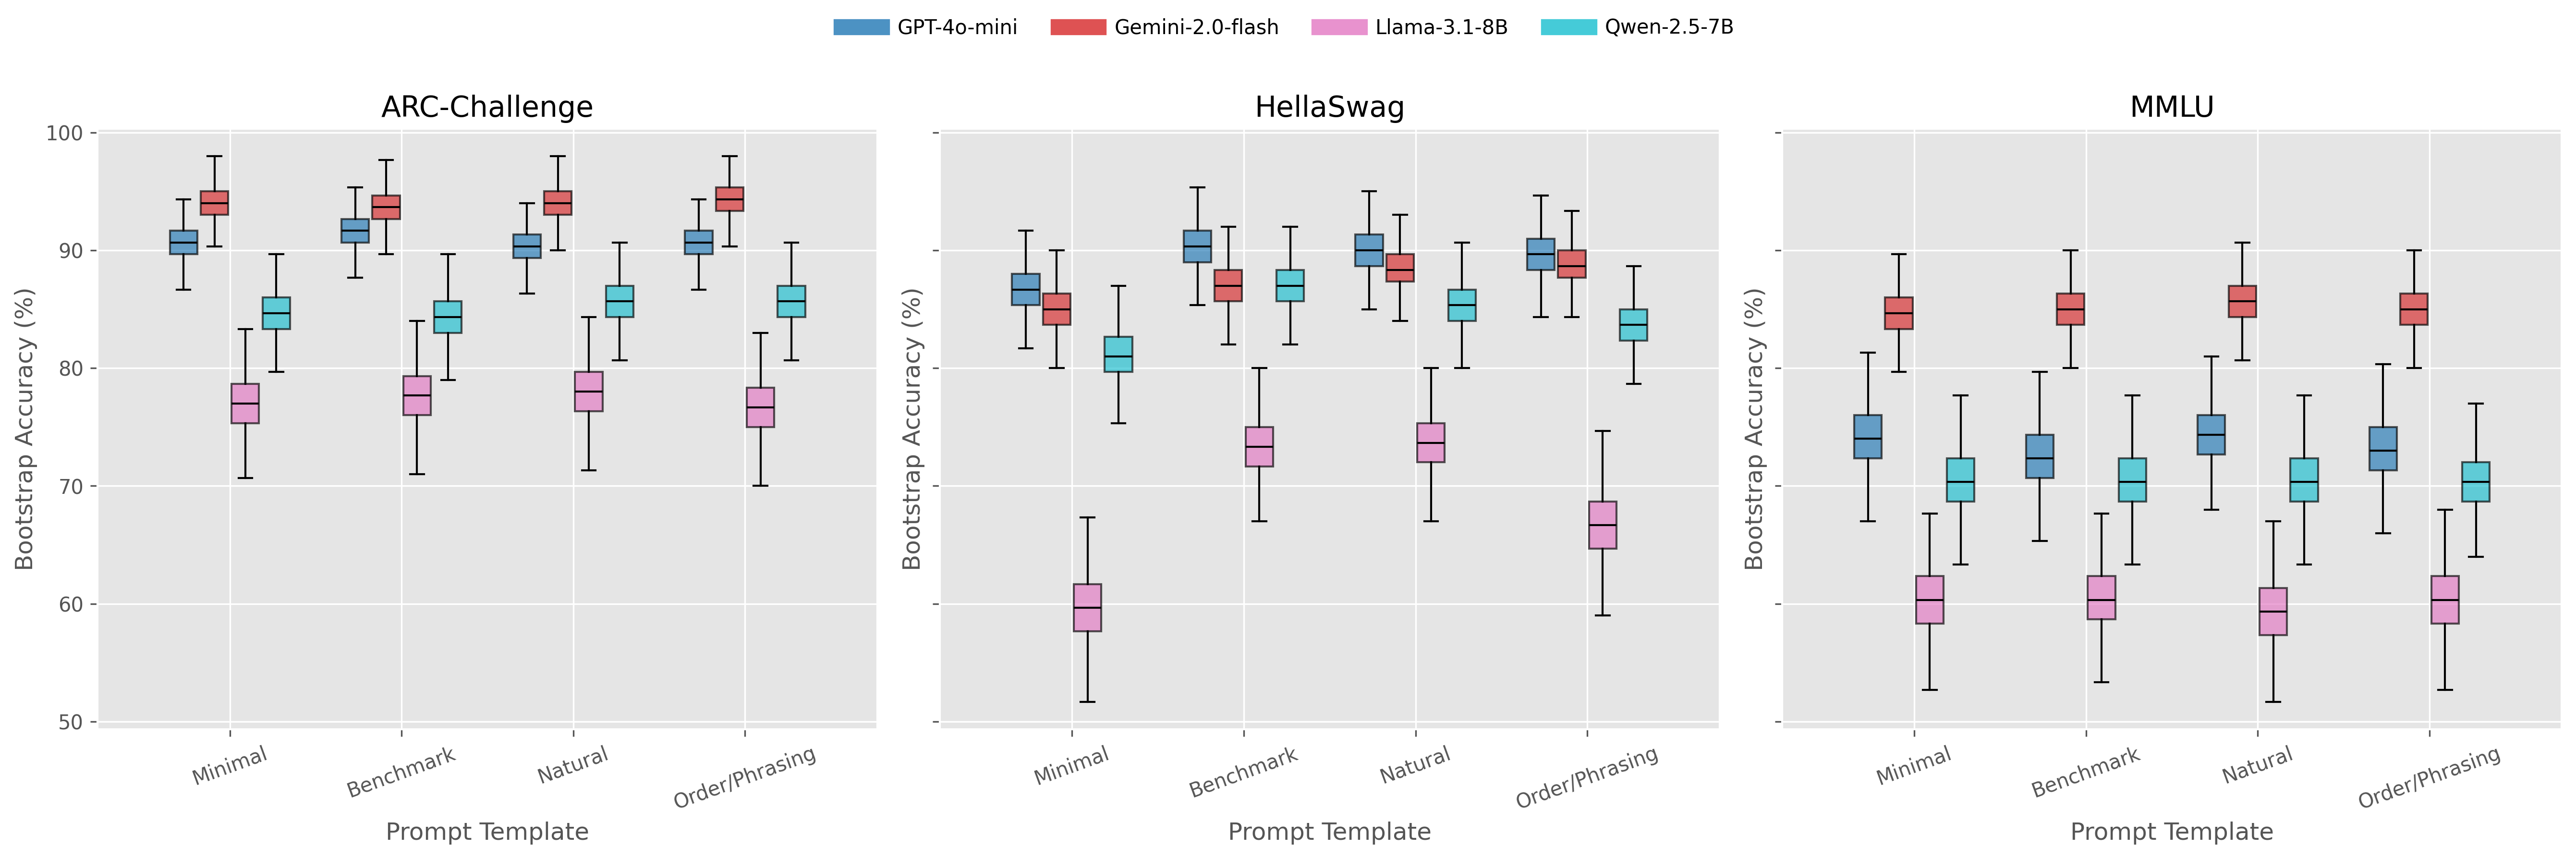
\includegraphics[width=\textwidth]{figures/accuracy_boxplots.png}
\caption{Bootstrap accuracy boxplots across prompt templates and benchmarks.}
\end{figure}

\begin{figure}[H]
\centering
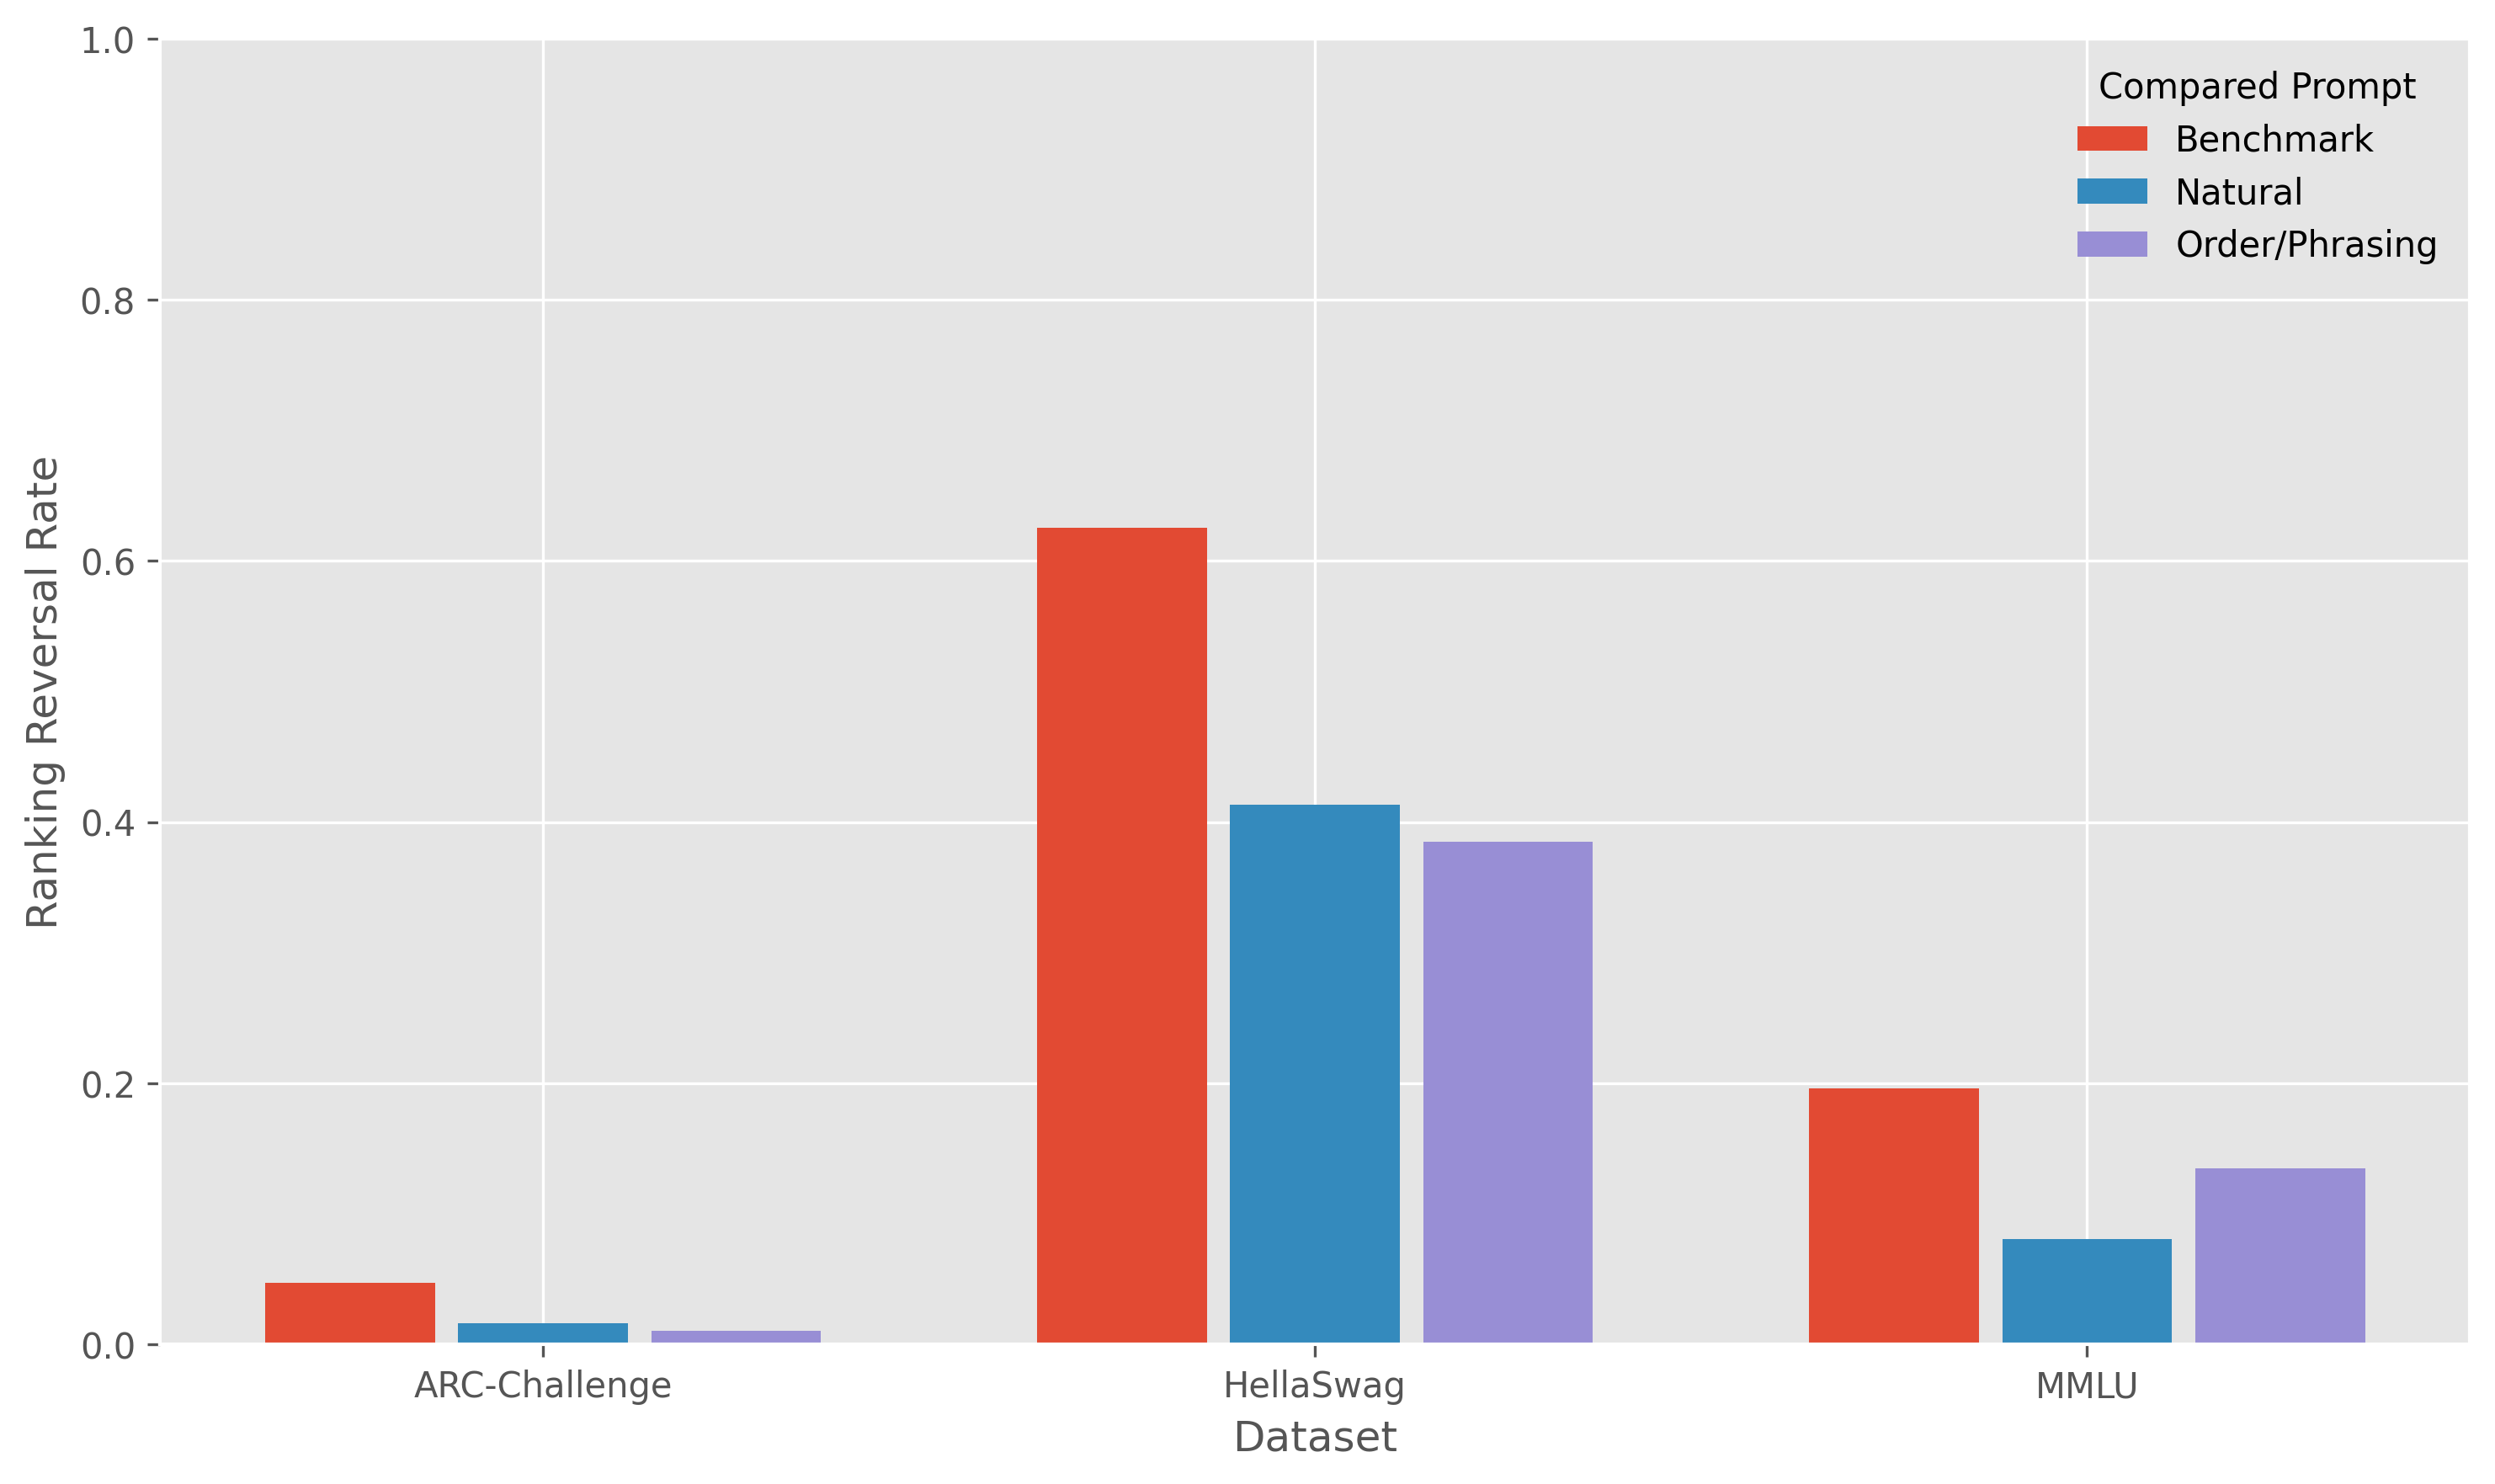
\includegraphics[width=0.72\textwidth]{figures/ranking_reversal_rate.png}
\caption{Ranking reversal rate relative to the minimal prompt.}
\end{figure}

\begin{figure}[H]
\centering
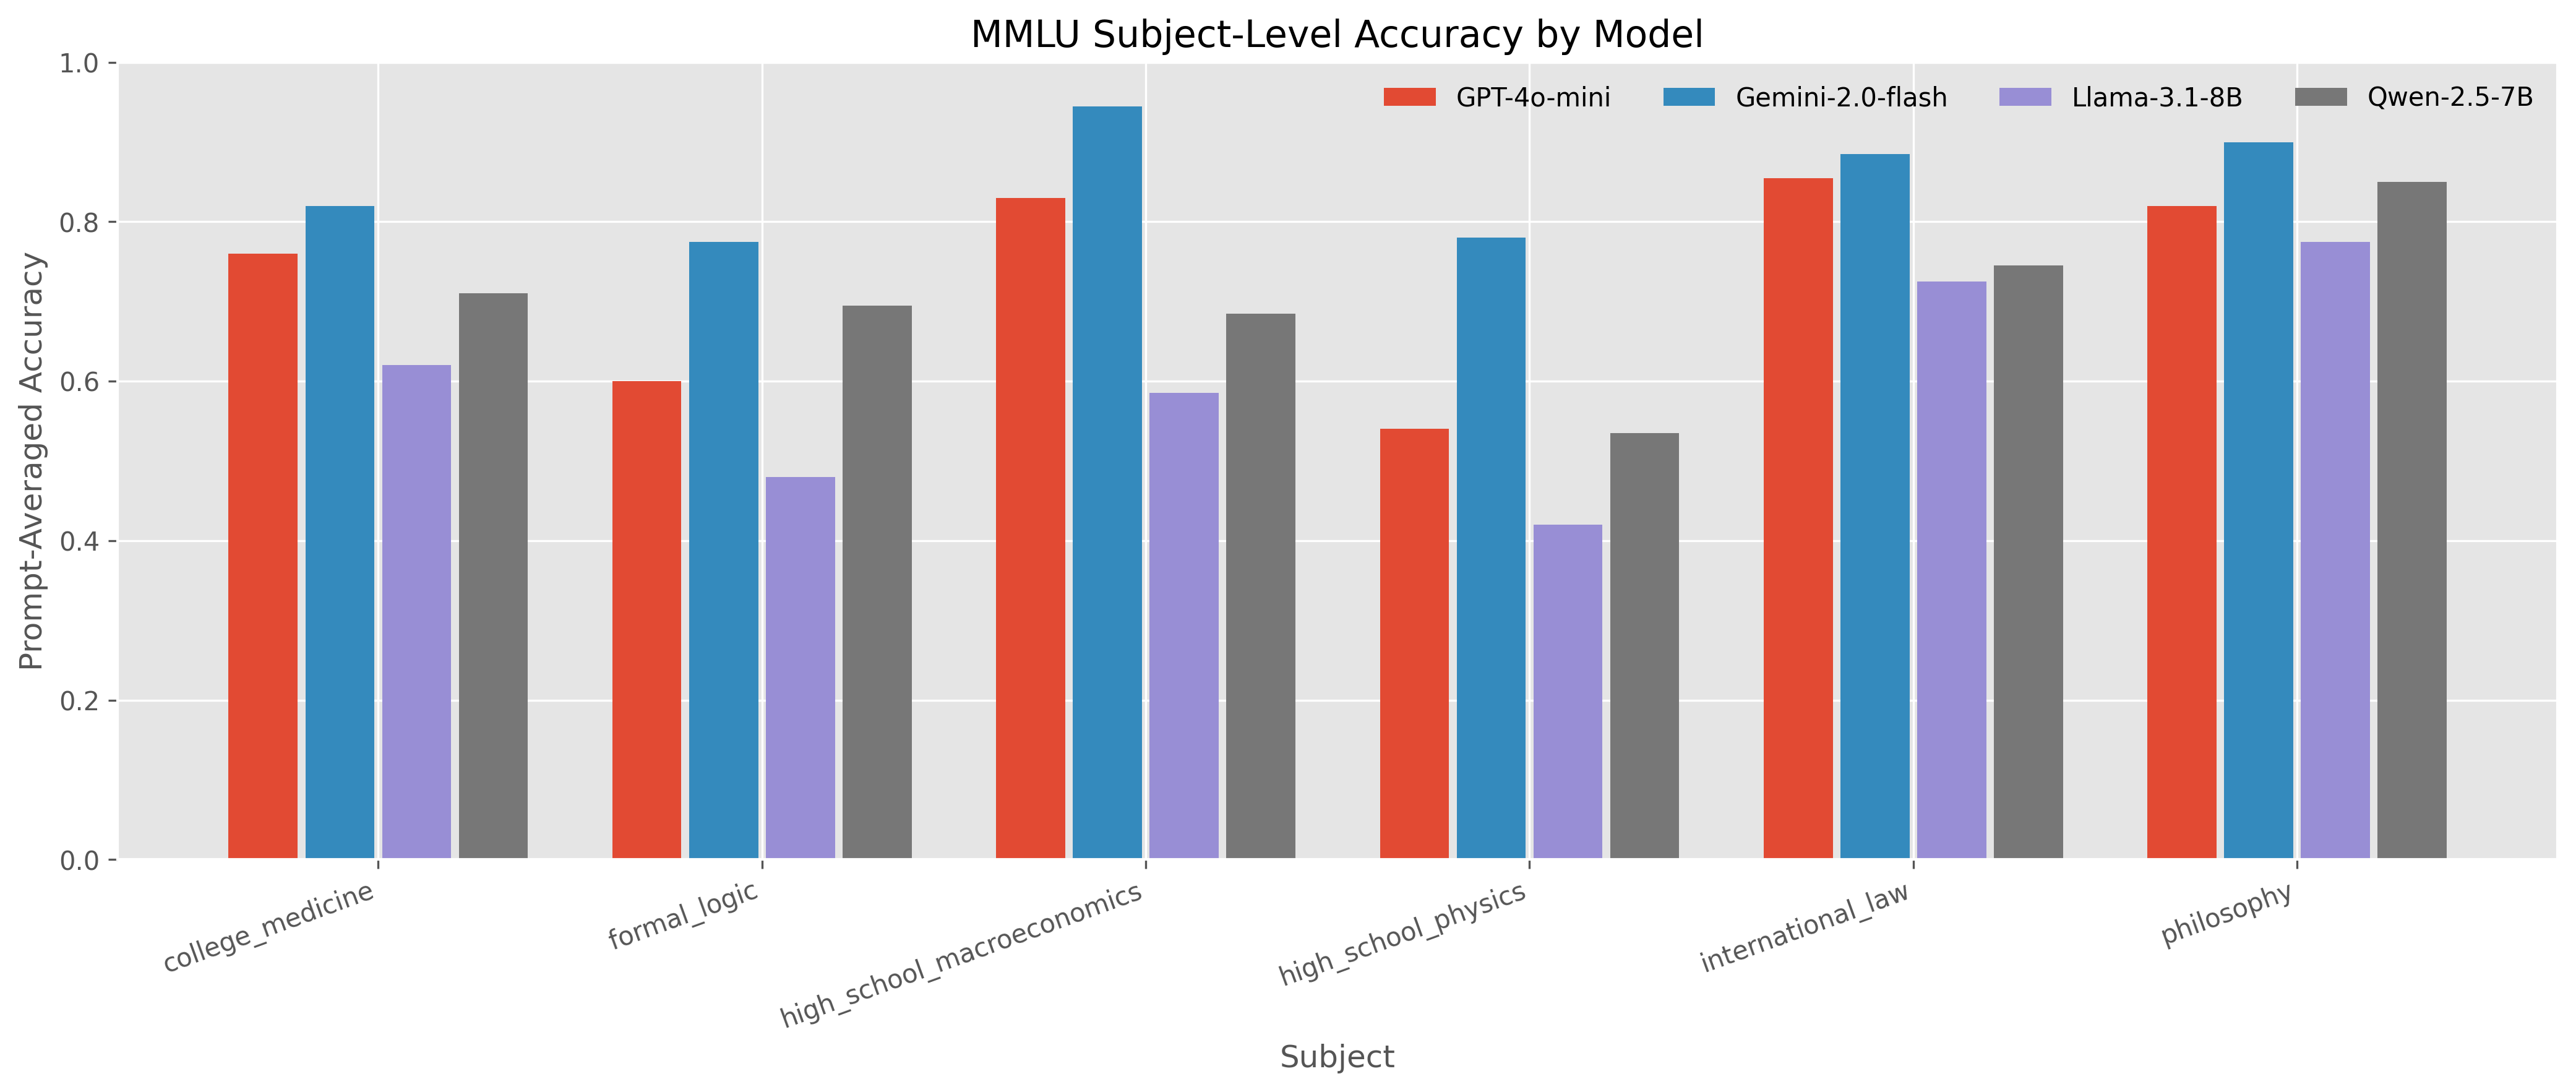
\includegraphics[width=\textwidth]{figures/mmlu_subject_accuracy.png}
\caption{MMLU subject-level prompt-averaged accuracy by model.}
\end{figure}

\begin{figure}[H]
\centering
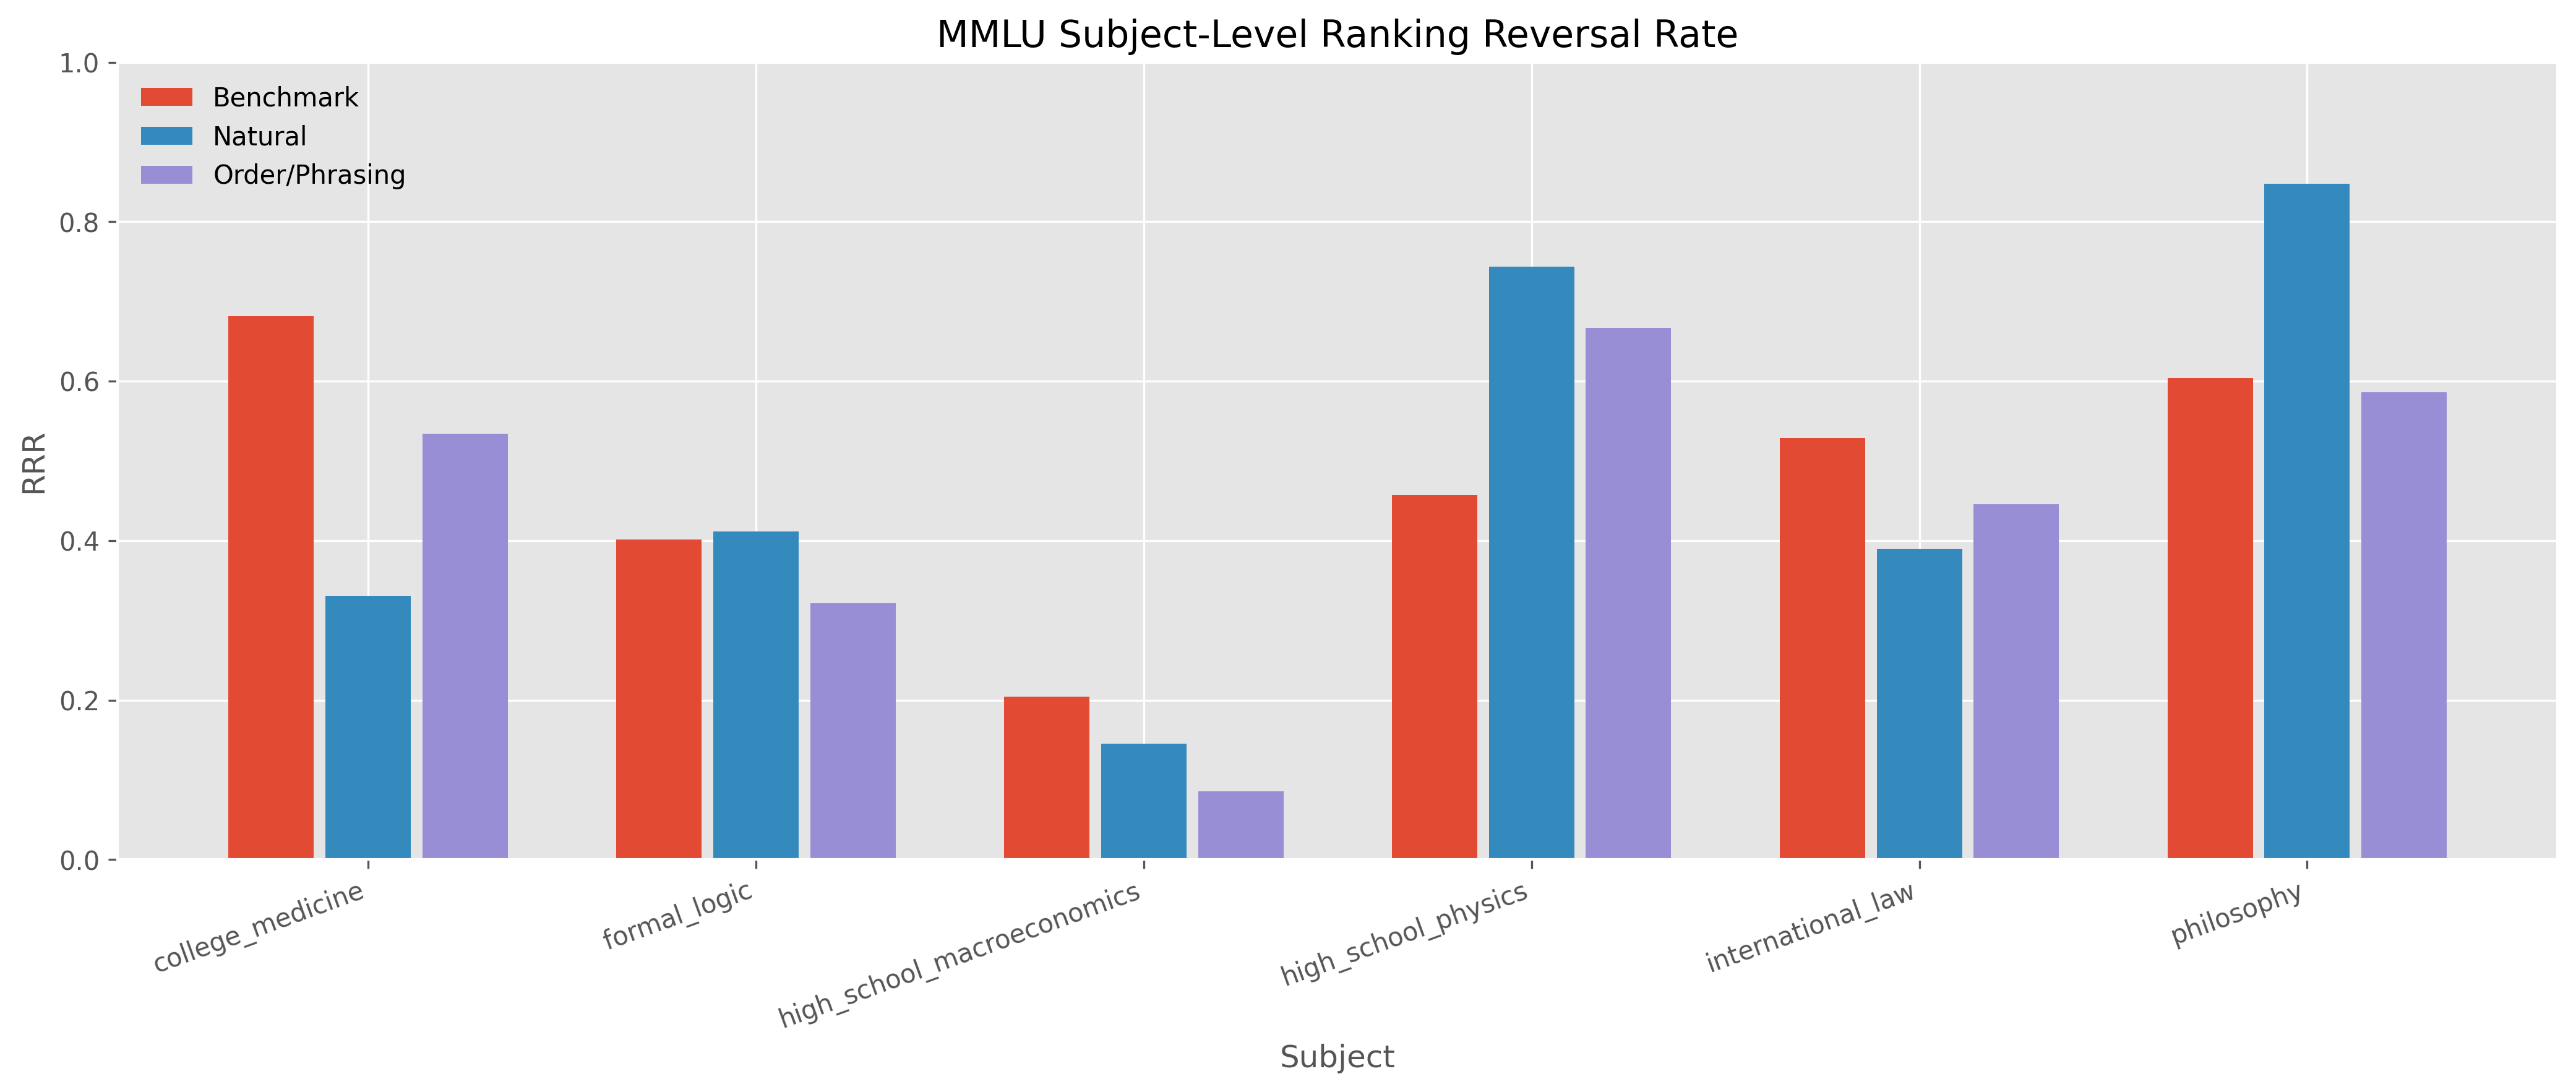
\includegraphics[width=\textwidth]{figures/mmlu_subject_rrr.png}
\caption{MMLU subject-level ranking reversal rate.}
\end{figure}

\begin{thebibliography}{9}
\bibitem{arc}
Clark, P., Cowhey, I., Etzioni, O., Khot, T., Sabharwal, A., Schoenick, C., and Tafjord, O.
\newblock Think You Have Solved Question Answering? Try ARC, the AI2 Reasoning Challenge.
\newblock 2018.

\bibitem{mmlu}
Hendrycks, D., Burns, C., Basart, S., Zou, A., Mazeika, M., Song, D., and Steinhardt, J.
\newblock Measuring Massive Multitask Language Understanding.
\newblock 2020.

\bibitem{hellaswag}
Zellers, R., Holtzman, A., Bisk, Y., Farhadi, A., and Choi, Y.
\newblock HellaSwag: Can a Machine Really Finish Your Sentence?
\newblock 2019.

\bibitem{promptrobust}
Zhu, K., Wang, J., Zhou, J., Wang, Z., Chen, H., Wang, Y., Yang, L., Ye, W., Gong, N. Z., Zhang, Y., and Xie, X.
\newblock PromptRobust: Towards Evaluating the Robustness of Large Language Models on Adversarial Prompts.
\newblock 2023.
\end{thebibliography}

\end{document}
